\documentclass[letterpaper,11pt]{article}
\usepackage{amsmath}
\usepackage{amsfonts}
\usepackage{listings}
\usepackage{tikz}

\usetikzlibrary{decorations.pathmorphing, positioning, arrows.meta, patterns, calc, decorations.markings}

%%%%%%%%%%%%%%%%%%%%%%%%%%%%%%%%%%%%%%%%5
%
%  Set Up Margins
\input{templates/pagedim.tex}

%%%%%%%%%%%%%%%%%%%%%%%%%%%%%%%%%%%%%%%%%%%%%%%%%%%
%
%    Minted package for nice python highlighting
%
\usepackage{minted}  % python syntax highlight

% Required packages

% Configure minted styling
\setminted[python]{
    frame=lines,
    framesep=2mm,
    baselinestretch=1.0,
    fontsize=\footnotesize,
    linenos=true,
    breaklines,
    %     style=monokai,
    style=default
}
\setminted[C]{
    frame=lines,
    framesep=2mm,
    baselinestretch=1.0,
    fontsize=\footnotesize,
    linenos=true,
    breaklines,
    %     style=monokai,
    style=default
}

% Configure listing to have a specific width
\setminted{
    numbersep=2pt,    % Distance between line numbers and code
    xleftmargin=20pt, % Left margin (increase if line numbers still overflow)
    xrightmargin=-2pt  % Right margin (decrease to reduce extra white space)
}
%
% % Configure listing caption style
% \DeclareCaptionFormat{listing}{\raggedright#1#2#3}
% \captionsetup[listing]{
%     format=listing,
%     labelfont=bf,
%     font=small,
%     labelsep=period
% }

%%%%%%% end of minted %%%%%%%%%%%%%%%%%%%%%%%%%%%%%%%%%%%%%%%%%%%%
\usepackage{mdframed}

\begin{document}
%
\begin{center}{\Large
Efficiency of resonant vibration generators\\
Blake Hannaford, Ph.D\\}
20-Jun-2025
\end{center}


\begin{figure}[b]\centering
% \documentclass{article}
% \usepackage{tikz}
% \usetikzlibrary{decorations.pathmorphing, positioning, arrows.meta, patterns, calc, decorations.markings}
%
% \begin{document}

\tikzset{
  % Remove unused pic definitions to avoid spurious text
}

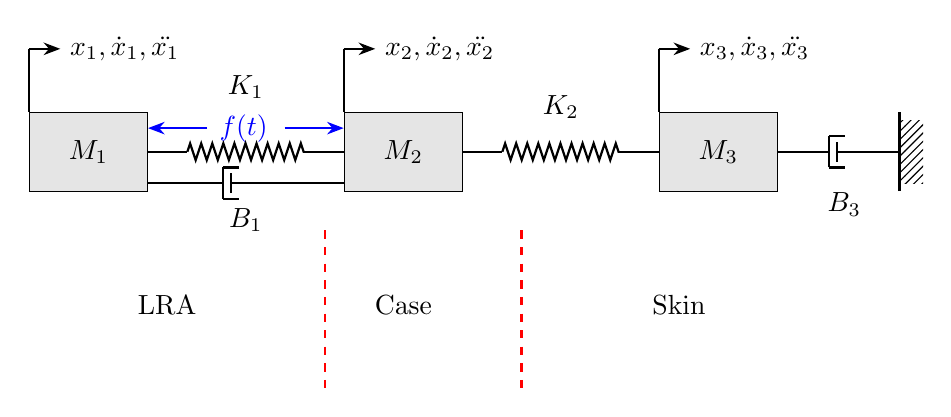
\begin{tikzpicture}[
    mass/.style={draw, rectangle, minimum width=1.5cm, minimum height=1cm, fill=gray!20},
    force/.style={-{Stealth[length=8pt]}, thick, red},
]

% Mass nodes
\node[mass] (M1) at (2,0) {$M_1$};
\node[mass] (M2) at (6,0) {$M_2$};
\node[mass] (M3) at (10,0) {$M_3$};

% Spring K₁ between M₁ and M₂
% No pic - draw directly connected to masses
\draw[thick] (M1.east) -- ++(0.5,0);
\draw[decoration={zigzag, segment length=4pt, amplitude=3pt}, decorate, thick]
      ([xshift=0.5cm]M1.east) -- ([xshift=-0.5cm]M2.west);
\draw[thick] ([xshift=-0.5cm]M2.west) -- (M2.west);
\node[above] at (4,0.55) {$K_1$};

% Damper B₁ between M₁ and M₂ (offset down) - draw directly connected
\draw[thick] ([yshift=-0.4cm]M1.east) -- ++(0.95cm,0);
% Damper symbol
\draw[thick] ([xshift=0.95cm,yshift=-0.6cm]M1.east) -- ++(0,0.4);     % outer vertical
\draw[thick] ([xshift=0.95cm,yshift=-0.2cm]M1.east) -- ++(0.2,0);  % upper outer horiz
\draw[thick] ([xshift=0.95cm,yshift=-0.6cm]M1.east) -- ++(0.2,0);  % lower outer horiz
\draw[thick] ([xshift=1.05cm,yshift=-0.525cm]M1.east) -- ++(0,0.25);   % inner vertical
% right horiz connector
\draw[thick] ([xshift=1.05cm,yshift=-0.4cm]M1.east)  -- ([yshift=-0.4cm]M2.west);
\node[below] at (4,-0.6) {$B_1$};

% Spring K₂ between M₂ and M₃
\draw[thick] (M2.east) -- ++(0.5,0);
\draw[decoration={zigzag, segment length=4pt, amplitude=3pt}, decorate, thick]
      ([xshift=0.5cm]M2.east) -- ([xshift=-0.5cm]M3.west);
\draw[thick] ([xshift=-0.5cm]M3.west) -- (M3.west);
\node[above] at (8,0.3) {$K_2$};

% Damper B₃ from M₃ to ground (centered on M3)
\draw[thick] (M3.east) -- ++(0.65cm,0);
% Damper symbol
\draw[thick] ([xshift=0.65cm,yshift=-0.2cm]M3.east) -- ++(0,0.4);     % outer vertical
\draw[thick] ([xshift=0.65cm,yshift=0.2cm]M3.east) -- ++(0.2,0);  % upper outer horiz
\draw[thick] ([xshift=0.65cm,yshift=-0.2cm]M3.east) -- ++(0.2,0);  % lower outer horiz
\draw[thick] ([xshift=0.75cm,yshift=-0.125cm]M3.east) -- ++(0,0.25);   % inner vertical
% right horiz connector to ground
\draw[thick] ([xshift=0.75cm]M3.east) -- (12.3,0);

% Ground at right (skin) - vertical line with hatching to the right
\draw[thick] (12.3,-0.5) -- (12.3,0.5);
\node[fill,pattern=north east lines,draw=none,minimum width=0.3cm,minimum height=0.8cm] at (12.45,0) {};
\node[below] at (11.6,-0.4) {$B_3$};

% Position indicators - vertical lines from upper left corners with horizontal arrows
% x₁
\draw[thick] (M1.north west) -- ++(0,0.8);
\draw[-{Stealth[length=6pt]}, thick] ([yshift=0.8cm]M1.north west) -- ++(0.4,0);
\node[right] at ([xshift=0.4cm,yshift=0.8cm]M1.north west) {$x_1, \dot{x}_1, \ddot{x_1}$};

% x₂
\draw[thick] (M2.north west) -- ++(0,0.8);
\draw[-{Stealth[length=6pt]}, thick] ([yshift=0.8cm]M2.north west) -- ++(0.4,0);
\node[right] at ([xshift=0.4cm,yshift=0.8cm]M2.north west) {$x_2, \dot{x}_2, \ddot{x_2}$};

% x₃
\draw[thick] (M3.north west) -- ++(0,0.8);
\draw[-{Stealth[length=6pt]}, thick] ([yshift=0.8cm]M3.north west) -- ++(0.4,0);
\node[right] at ([xshift=0.4cm,yshift=0.8cm]M3.north west) {$x_3, \dot{x}_3, \ddot{x_3}$};

% f(t) force arrows
\draw[thick, blue, -{Stealth[length=6pt]}] ([xshift= 0.75cm,yshift=0.3cm]M1.east) -- ([xshift=0.0cm,yshift=0.3cm]M1.east);
\draw[thick, blue, -{Stealth[length=6pt]}] ([xshift=-0.75cm,yshift=0.3cm]M2.west) -- ([yshift=0.3cm]M2.west);
\node[left, blue] at (4.4,0.3) {$f(t)$};

% Bottom labels
\node[below] at (3,-1.7) {LRA};
\draw[thick, red, dashed]  (5,-1.) -- (5,-3);
\node[below] at (6,-1.7) {Case};
\draw[thick, red, dashed]  (7.5,-1.) -- (7.5,-3);
\node[below] at (9.5,-1.7) {Skin};

\end{tikzpicture}

% \end{document}

\caption{}\label{3MassSchematic}
\end{figure}

\section*{Introduction}
This is a basic study of energy flows in a resonant system.  A typical application could be a Linear Resonant Actuator (LRA), inside a cellphone case,
held in the fingers.  The objective is to transfer vibration energy into the fingers to create haptic sensations.   Among the questions we will
attempt to answer are:
\begin{enumerate}
    \item  What is a useful dynamical model and simulation for such a system? What are some reasonable parameter values?
    \item  What are flows of energy which can be quantified in such a system?
%     \item  Only damping elements can dissipate energy. Springs and Masses can only store and return energy.   In the steady state (after starting
%     transients), the total energy stored in all masses (kinetic energy) and springs (potential energy), will therefore be constant.  Therefore, we
%     can ask, what is the dissipation of energy in the two dampers (friction loss elements) $B_1$ the LRA damping, and $B_3$ the damping of the skin
%     model.
    \item A significant practical issue is to ensure the accuracy of our energy computations with respect to numerical errors which may
    occur in simulation algorithms, particularly related to energy balance and conservation of energy.    All energy into the system must
    be properly accounted for as either dissipation in damping elements or residual energy in the storage components (Mass, Springs) at the end of the simulation.
    \item  What is a suitable experiment to simulate with such a computational model to study efficiency of
    actuation for vibrotactile haptics.
     With the above questions answered we can ask the main question:

         ``is an an electromagnetic
     actuator with vibration output more efficient if it is a resonant system?''

     and, relatedly,

     ``If it is resonant, is it more efficient when driven at its resonant frequency?''
\end{enumerate}

\section{Q1: What is a useful dynamical model and simulation for such a system? What are some reasonable parameter values?}

We introduce the model of Figure \ref{3MassSchematic}.  Three masses represent in turn, the mass of the moving LRA component ($M_1$),
the mass of static LRA components, as well as all other static components of a hand held device including battery (my Pixel 6a phone
has a total weight of about 250 grams) is encompassed in $M_2$ which we assume is a rigid body.
$K_2, M_3, B_3$ represent a simplified model of skin at frequencies of about 150 Hz which is
near the most sensitive frequency of human skin and is widely used in haptic signals.

Using standard techniques for dynamical system analysis, we derived a mathematical model of this system which accepts a time varying force
applied to the LRA mass and the case in equal and opposite directions (Appendix).   Any force or motion within the system can be an output which we can
analyze as a result of the applied force.  We can also compute energy flows among the components of this system.

\subsection{Model Parameter Values}
LRA properties can be directly measured by dissection of LRA devices.  Mass is simplest to obtain by weighing, spring constants can be measured by
compression testing, and damping can be measured by dynamic tests.   Resonance behavior of real devices can be conveniently tested by observing
a voltage transient on it's actuator when the device is tapped on a table.   With one measured parameter, the others can be inferred from the
frequency ($\omega_n$) and decay time (damping) of the tapping transient.

The biomechanics of skin are complex but here we rely on a previously published study which surveyed skin models in the literature to
derive consensus model parameters for a single point of contact for vibrotactile haptic signal response of skin\footnote{Lindsay, Jack, Richard J. Adams, and Blake Hannaford. ``Improving tactile feedback with an impedance adapter.'' In 2013 World Haptics Conference (WHC), pp. 713-718. IEEE, 2013.
}.
\paragraph{Masses:}
Mass of the LRA moving weight is taken from a typical device characterized in the (Lindsay et al., 2013) reference.   Mass of the case was
obtained by weighing a typical cell phone (Pixel 6a).   Mass of the skin used the same reference but was multiplied by 4 based on the assumption of
4 fingers contacting the phone body simultaneously via 4 skin patches.

\paragraph{Springs:}
LRA constant $K_1$ is derived from the LRA moving mass and the desired resonant frequency
which we held constant at 150 Hz.  Skin spring constant
$K_2$ is also  taken from the reference.

\paragraph{Dampers:}
LRA Damping $B_1$ was derived from $K_1$ by assuming a damping ratio, $\zeta$, according to the degree of resonant behavior expected in the device.
For $\zeta=1$, there is no resonant behavior, and as $\zeta$ approaches zero, the system is more and more resonant.  We used a value of $\zeta=0.01$
to represent a typical LRA value of damping.

The resulting parameters are:
\begin{table}[h]
\centering
\begin{tabular}{|l|l|p{1.25in}|p{1.05in}|}\hline

\textbf{Name} & \textbf{Description} & \textbf{Value/Equation} & {\bf Source}\\
\hline
$\omega_n$   &  LRA resonant Frequency &  150  $rad/sec$ & Assumption \\\hline
$\zeta$      &  LRA damping ratio      &   0.01          & Assumption \\\hline
M1 & LRA mass & 0.005 $kg$  & [1]\\
\hline
K1 & LRA spring constant & $\omega_n^2   M1$ & [1]\\
\hline
B1 & LRA damping coefficient & $\zeta   2\sqrt{K_1M_1}$ & Derived based on assumed $\zeta$.\\
\hline
M2 & Case mass & 0.2250 $kg$ & Pixel 6a weight\\
\hline
$n_{contact}$  &  Number skin contacts & 4 & Nominal grasp of phone case \\
\hline
K2 & Skin spring constant & $n_{contact}   K_{skin}$ & [1] \\
\hline
B3 & Skin damping coefficient & $n_{contact}   B_{sk}$ & [1] \\
\hline
M3 & Skin mass & $n_{contact}   M_{sk}$ &  $ [1] $ \\
\hline
$K_{skin}$ & Single contact skin stiffness & 300 N/m & [1] \\
\hline
$B_{sk}$ & Single contact skin damping & $1.6$ Nsec/m & [1]\\
\hline
$M_{sk}$ & Single contact skin mass    & $0.01*M1$    & a negligible value, $kg$ [1] \\
\hline
\end{tabular}
\end{table}

\subsection{Model Simulation}

The dynamical model of the Appendix was converted to state space (Matrix) form and simulated with a python program using the {\tt python.control} package
(Listings \ref{Listing1} and ref{Listing2} below).
Input force signals were modeled by a sinusoid function.
To implement this drive in a real LRA, a sinusoidal current would be applied to the
actuator coil or coils.  Rectangular current pulses of any frequency or amplitude can also be simulated.

Python code, using the {\tt python.control} module to simulate such a model and computer energy flows and
totals, is given in Listing 1.



\section{Q2: What are flows of energy which can be quantified in such a system?}
\label{WhatAreEnergyFlows}

When a mass $M$ is driven by a force $f(t)$ it moves according to Newtonian mechanics.  The amount it moves depends on the values of various
parameters such as Masses, Springs, etc.    When a force is applied, work may be done on the load according to
\[
W = f(t)\Delta x
\]
over a time interval $T$, the energy (Joules)
delivered to the load (or absorbed from the load) is
\[
E = \int_0^T f(t)x(t)dt
\]
Thus we can compute energy flows at any connection in the system where force and displacement are known.

Energy flows of particular interest include total energy flowing out of the force generator represented by $f(t)$, and
total energy dissipation (conversion of energy to heat) taking place in the damper elements.
We consider several energy flows below:

\subsection{Actuator Output}   develops between case and LRA mass. Thus
    it is applied by the actuator at two points and in two directions
    (coil mass is lumped into Case mass) and there are two components:
    \[
    E_{so} = E_1 + E_2 = \sum_t \left[ -f(t) \Delta x_1 + f(t)\Delta x_2 \right]
    \]
    where
    \[
    \Delta x_i = \dot{x}_i\Delta t
    \]
    (We have written this expression in discrete time to allow easy adaptation to
    simulation output data every $\Delta t$ seconds.)


\subsection{LRA Damping Loss}
    (lost energy in $B_1$) is
    \[
    f_{B1} = (\dot{x}_2-\dot{x_1})B_1
    \]
    \[
    \Delta x_{B1} = (\dot{x}_2-\dot{x}_1)\Delta t
    \]
    giving
    \[
    E_{B1} = \sum_t B_1(\dot{x}_2-\dot{x}_1)^2\Delta t
    \]

\subsection{Energy input to the case}  from the actuator is
    \[
    E_{ca} = \sum_t  f(t)\Delta x_2
    \]


\subsection{Output to Skin} will be interpreted as  work done on
    (deformation of) the skin stiffness ($K_2$) as
    \[
    E_{sk} = K_2(x_2-x_3)\dot{x}_2 \Delta t
    \]

\subsection{Energy Dissipation in Skin ($B_3$)}
    Since only one end of the skin damper is moving, we have a simpler form than the LRA damper:
    \[
    E_{B3} = B_3\dot{x}_3^2\Delta t
    \]


\section{Q3: How well is energy conserved in the numerical simulation computations?}

In the steady state, the energy input to the system must be equal to the energy dissipated in the two
dampers since masses and springs can only store and release energy.  However, numerical bookeeping
errors (known as ``energy leaks'') can arise if numerical precision is not sufficient.  Thus we
numerically compared
\[
E_{leak} = E_{so} - E_{B_1} - E_{B_3}
\]
for a period of time after the system reaches steady state vibration. Ideally $E_{leak}=0$, but we will
strive to keep it such that
\begin{equation}\label{EqnEnergyBalance}
|E_{leak}| < 0.01 E_{so}
\end{equation}


\section{Q4: What are suitable experiments for answering the above questions?}

Computational experiments with this model fall into two classes 1) model validation and 2)
hypothesis testing.

Model validation will consist of verification of Eqn \ref{EqnEnergyBalance}.

Two questions amount to hypothesis testing:
\subsection{}\label{ResQ1}
\begin{quotation}  All other parameters being equal, is a system that is resonant ($0<\zeta<1.0$) more ``efficient''
compared to a system that is non-resonant ($\zeta=1.0$)?
\end{quotation}

And, a related question is:
\subsection{}\label{ResQ2}
\begin{quotation}
If resonant systems  $S_1$ and $S_2$ have damping ratios $\zeta_1$ and $\zeta_2$ respectively, if
$0<\zeta_1 < \zeta_2<1$, is $S_1$ more efficient?
\end{quotation}

A simpler question which is not the same as efficiency, is,
\subsection{}\label{ResQ3}
\begin{quotation} Given a fixed force input signal,
does a resonant  ($0<\zeta<1.0$)  system have a greater output (displacement or energy)?
\end{quotation}


\paragraph{Efficiency}
With full consideration of Question Q\ref{WhatAreEnergyFlows}, it becomes
clear that conservation of energy requires that all energy dissipated in the
dampers $(B_1, B_3)$ to be supplied by the energy source under all steady state conditions.
Transiently, as energy enters or leaves the combined mass-spring system, damper dissipation
will not be equal to source energy.

Furthermore,
greater motion of the masses drives greater energy dissipation in the dampers.

Assuming we define efficiency as
\[
ee = \frac {E_{sk}}  {E_{so}} = \frac {\mathrm{E~to ~skin} } { \mathrm {E~from~source} }
\]
there is
no free lunch, and if resonant systems have a higher output energy it must be
in direct proportion to increased energy drawn from their power source.

Nevertheless, if ``efficiency'' may have other definitions such as

\[
eo = \frac {O_{sk}}  {F_{so}} = \frac {\mathrm{Output~to ~skin} } { \mathrm {Force~from~source} }
\]
where output is, for example RMS skin surface deformation or velocity
we consider a force or displacement variable instead of energy.

We can simulate various inputs and compute the above efficiencies, $ee, eo$.

We define the following computational experiment:

\begin{enumerate}
    \item Define our parameters and constants of the system. We specify the resonant
    frequency of the LRA components to be 150Hz, $K_1, M_1$ and derive $K_1$ accordingly.

    \item While $\omega_n = 150\times2\pi$ of the physical system
    is held constant, we define a range of test
    frequencies at which to drive the system:
        \[
            0.95 \omega_n < \omega < 1.05 \omega_n
            \]
        having $npar$ discrete values, as well as a range of $npar$ system damping ratios:
            \[
                0.01 < \zeta < 1.0
                \]
    We set $npar=10$.

    \item For each pair $\omega_i, \zeta_i$, we simulate the system for
    \[
    400 \mathrm{cycles}\times 150 Hz = 2.67 \mathrm(sec)
    \]
    and compute the various  amplitudes and energy flows.
    To avoid transient effects, we compute the energy flows over only the final 25\%
    of the simulation time.

    \item Plot the result as a heatmap.

\end{enumerate}

xxxxxxxxxxxxxxxxxxxxxxxxxxxxxxxxxxxxxxxxxxxxxxxxxxxxxxx

xxxxxx



\section{Computational Results}

We first address the issue of energy bookeeping.  Using the above workflow, we
first computed $E_{leak}$ expressed as a percentage of the actuator output energy,
$eso$ (Figure \ref{EleakFig}).   We see that energy leakage is below 1.2\%
for all combinations, with the larger errors evident for less resnonant
systems ($\zeta \to 1.0$).


\begin{figure}
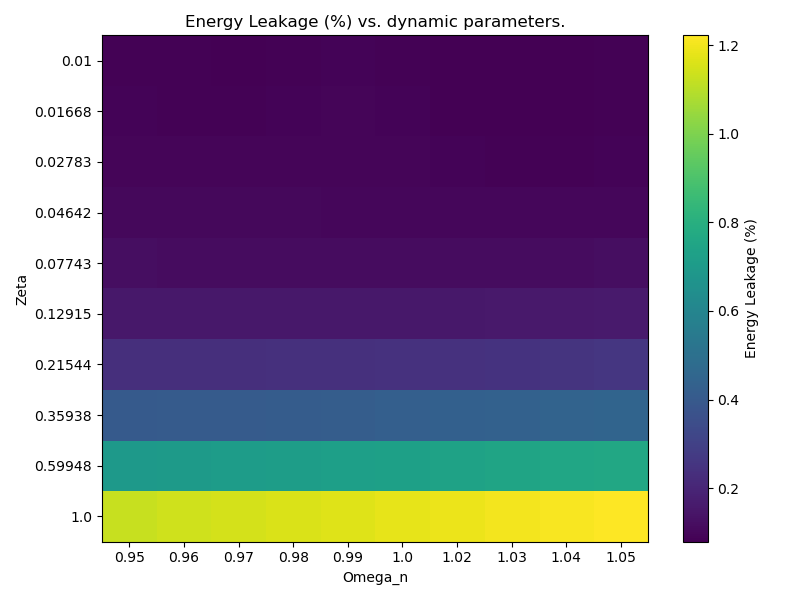
\includegraphics[width=0.5\textwidth]{heatmapleakage_10x10.png}
\caption{}\label{EleakFig}
\end{figure}


Energy delivered to the skin (Figure \ref{SkinEFig}) has it's highest value at the resonant
frequency ($\omega=\omega_n$) and with the lowest value of
$\zeta$ as expected, but also interestingly may show higher outputs
just below the resonance than just above it.   This needs to be checked
for in case it's an artifact of the chosen $\omega, \zeta$ values.


\begin{figure}
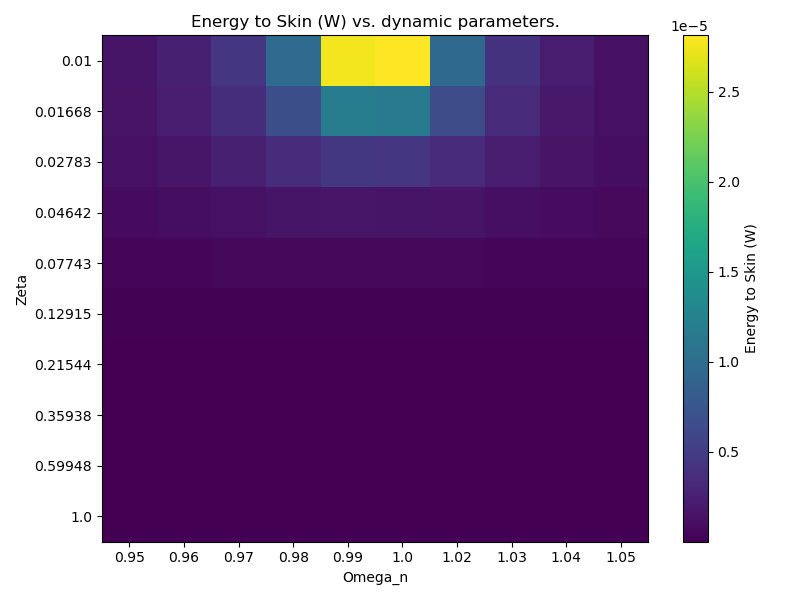
\includegraphics[width=0.5\textwidth]{heatmap_SkinE_10x10.png}
\caption{}\label{SkinEFig}
\end{figure}

Actuator energy output shows (Figure \ref{EoutFig}) a similar pattern to skin energy,
sharply peaking at the resonant frequency.


\begin{figure}
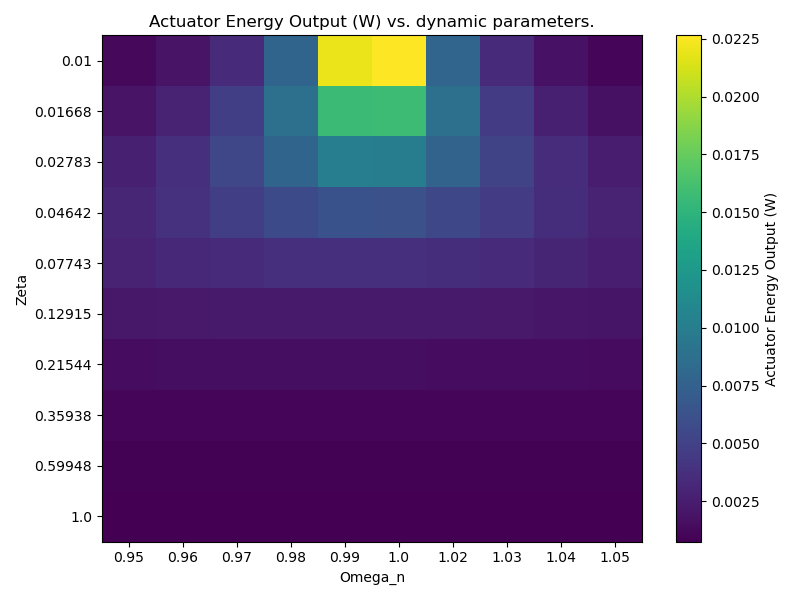
\includegraphics[width=0.5\textwidth]{heatmap_actOutput_10x10.png}
\caption{}\label{EoutFig}
\end{figure}

Now we address efficiency: $ee$ in terms of energy to skin vs. actuator output energy
(Figure \ref{EEficFig}).



\begin{figure}
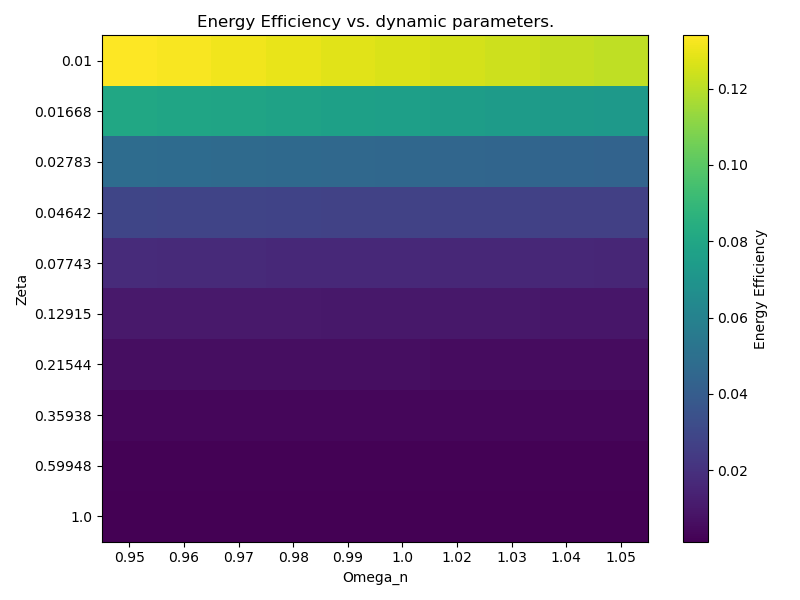
\includegraphics[width=0.5\textwidth]{heatmap_ee_10x10.png}
\caption{}\label{EEficFig}
\end{figure}




\begin{figure}
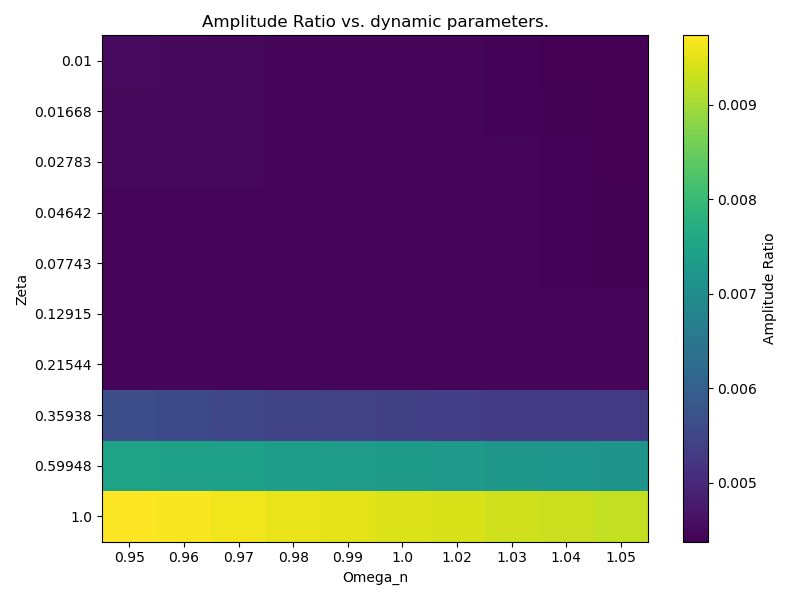
\includegraphics[width=0.5\textwidth]{heatmap_gain_10x10.png}
\caption{}\label{GainFig}
\end{figure}



\clearpage
\newpage\section*{Appendix: Derivation of mathematical model}
\noindent \textbf{System Parameters}

\begin{table}[h]
\centering
\begin{tabular}{|l|l|l|}
\hline
\textbf{Name} & \textbf{Description} & \textbf{Value/Equation} \\
\hline
M1 & LRA mass & 0.005 kg \\
\hline
K1 & LRA spring constant & $\omega_n^2   M1$ \\
\hline
B1 & LRA damping coefficient & 2 $\zeta   \sqrt{K1   M1}$ \\
\hline
M2 & Case mass & 0.2250 kg \\
\hline
K2 & Skin spring constant & $n_{contact}   K_{skin}$ \\
\hline
B3 & Skin damping coefficient & $n_{contact}   B_{sk}$ \\
\hline
M3 & Skin mass & $n_{contact}   M_{sk}$ \\
\hline
$K_{skin}$ & Single contact skin stiffness & 300 N/m \\
\hline
$B_{sk}$ & Single contact skin damping & $\frac{0.75 + 2.38}{2}$ Nsec/m \\
\hline
$M_{sk}$ & Single contact skin mass & $0.01   M1$ kg \\
\hline
\end{tabular}
\end{table}


\noindent \textbf{Force Balance}

\[
M_1 \ddot{x}_1 + B_1(\dot{x}_1 - \dot{x}_2) + K_1(x_1 - x_2) = -f(t)
\]

\[
M_2 \ddot{x}_2 + B_1(\dot{x}_2 - \dot{x}_1) + K_1(x_2 - x_1) + K_2(x_2 - x_3) = f(t)
\]

\[
M_3 \ddot{x}_3 + B_2 \dot{x}_3 + K_2(x_3 - x_2) = 0
\]

\noindent \textbf{State Vector} = $[x_1 \quad \dot{x}_1 \quad x_2 \quad \dot{x}_2 \quad x_3 \quad \dot{x}_3]^T$

\noindent \textbf{EOM 1}
\[
M_1 \ddot{x}_1 = -B_1(\dot{x}_1 - \dot{x}_2) - K_1(x_1 - x_2) - f(t)
\]

\[
\ddot{x}_1 = -\frac{K_1}{M_1} x_1 - \frac{B_1}{M_1} \dot{x}_1 + \frac{K_1}{M_1} x_2 + \frac{B_1}{M_1} \dot{x}_2 + 0   x_3 + 0   \dot{x}_3 - \frac{f(t)}{M_1}
\]

\noindent \textbf{EOM 2}
\[
M_2 \ddot{x}_2 = -B_1(\dot{x}_2 - \dot{x}_1) - K_1(x_2 - x_1) - K_2(x_2 - x_3) + f(t)
\]

\[
\ddot{x}_2 = \frac{K_1}{M_2} x_1 + \frac{B_1}{M_2} \dot{x}_1 - \frac{K_1 + K_2}{M_2} x_2 - \frac{B_1}{M_2} \dot{x}_2 + \frac{K_2}{M_2} x_3 + 0   \dot{x}_3 + \frac{f(t)}{M_2}
\]

\noindent \textbf{EOM 3}
\[
M_3 \ddot{x}_3 = -B_2 \dot{x}_3 - K_2(x_3 - x_2)
\]

\[
\ddot{x}_3 = 0   x_1 + 0   \dot{x}_1 + \frac{K_2}{M_3} x_2 + 0   \dot{x}_2 - \frac{K_2}{M_3} x_3 - \frac{B_2}{M_3} \dot{x}_3
\]

\[
\dot{X} = A X
\]

\[
\begin{bmatrix}
\dot{x}_1 \\
\ddot{x}_1 \\
\dot{x}_2 \\
\ddot{x}_2 \\
\dot{x}_3 \\
\ddot{x}_3
\end{bmatrix}
=
\begin{bmatrix}
0 & 1 & 0 & 0 & 0 & 0 \\
-\frac{K_1}{M_1} & -\frac{B_1}{M_1} & \frac{K_1}{M_1} & \frac{B_1}{M_1} & 0 & 0 \\
0 & 0 & 0 & 1 & 0 & 0 \\
\frac{K_1}{M_2} & \frac{B_1}{M_2} & -\frac{K_1+K_2}{M_2} & -\frac{B_1}{M_2} & \frac{K_2}{M_2} & 0 \\
0 & 0 & 0 & 0 & 0 & 1 \\
0 & 0 & \frac{K_2}{M_3} & 0 & -\frac{K_2}{M_3} & -\frac{B_2}{M_3}
\end{bmatrix}
\begin{bmatrix}
x_1 \\
\dot{x}_1 \\
x_2 \\
\dot{x}_2 \\
x_3 \\
\dot{x}_3
\end{bmatrix}
+
\begin{bmatrix}
0 \\
-\frac{1}{M_1} \\
0 \\
\frac{1}{M_2} \\
0 \\
0
\end{bmatrix}
f
\]

%
%   Code Listings below
\clearpage
\newpage
\begin{listing}[h]
    \caption{Python functions supporting the simulation and energy study.}\label{Listing1}
\end{listing}
\begin{minted}[linenos, fontsize=\small, frame=lines]{python}
import numpy as np
import seaborn as sns
import matplotlib.pyplot as plt
import sys
import control as ctl
import LRAsim as LRA
import heatmap as hm


TRAPEZOIDAL = LRA.TRAPEZOIDAL  # numerical integration method for energy


# get command line args:

if len(sys.argv) == 2:
    if sys.argv[1]=='plot':
        fname = input('enter heatmap filename: ')
        hm.hmap(fname.strip(),legend='Skin Dissipation ')
        quit()
    else:
        print('unknown argument: ', sys.argv[1])
        quit()

# get the energy flows

def RepHeatmap(wn,z, fd, heat):
    print(f'{wn:10.2f}, {z:10.5f}, {heat:.3e}', file=fd)

def Report2(wn,z, fd, eso, eca, elm, eld, ebs, Etot,yp):
    leakage = eso-(eld+ebs)
    plk = 100*leakage/eso
    print(f'{wn:10.2f}, {z:10.5f}, {eso:.3e}, {leakage:.3e}, {plk:8.1f}', file=fd)

nwn = 5
nzet = 5
fres = 150 # hz
wres = 2*np.pi*fres

wnv = np.geomspace(0.95*wres, 1.05*wres, num=nwn, endpoint=True)
zetav = np.geomspace(0.01, 1.0, num=nzet, endpoint=True)

dt = LRA.dt

fhz = fres
per = 1/fhz
Tmax = 400*per  # let's model 6 cycles

T = np.arange(0,Tmax,dt)
npts = len(T)

ncontact = 4  # four fingers touching (x4 skin model)
Ain = 1  # input amplitude (N)

sd={}
# sd['studytype'] = 'leakage'
# sd['legend']    = 'Energy Leakage (%)'
# sd['studytype'] = 'eout'
# sd['legend']    = 'Actuator Energy Output'
sd['studytype'] = 'SkinE'
sd['legend']    = 'Energy to Skin'

fname = f'heatmap{sd['studytype']}.csv'
dataf = open(fname, 'w')

#
#   input force to LRA
#
# Sin wave
# U = Ain*np.sin(wres*T)

# short rectangular pulses
U = np.zeros(len(T))
pf = 1/fres
p  = int(pf/dt)

for i,u in enumerate(U):
    if i%p==0:
        U[i] = Ain
    if (i+1)%p==0:
        U[i] = Ain
    if (i+2)%p==0:
        U[i] = Ain

dpar = {}
#  for all the wn and zeta possibilities:
#
for wn in wnv:
    for zetaLRA in zetav:
        #
        #   Simulate and analyze energy
        #

        # LRA properties
        M1 = 0.005 # kg   ()
        dpar['M1'] = M1
        # B1 = 0.03222  # Nsec/m
        K1 = wn**2 * M1
        dpar['K1'] = K1

        B1 = zetaLRA*2*np.sqrt(K1*M1)
        dpar['B1'] = B1

        print(f' Derived K1 ratio: {K1/2800:5f} vs 2800')
        # K1 = 2800  # N/m # (ref Jack's paper)

        # Case Properties
        Mc = 0.2250   # 225gr
        M2 = Mc
        dpar['M2']=M2

        # Skin Properties
        Kskin = 300 # N/m   (600-1200)
        K2=ncontact*Kskin     #
        dpar['K2'] = K2
        Bsk = (0.75+2.38)/2  # Nsec/m (0.75-2.38)
        # Bl = (2.38)  # Nsec/m (0.75-2.38)
        B3 = ncontact*Bsk
        dpar['B3']=B3

        Msk = 0.01 * M1  # essentially zero
        M3 = ncontact*Msk
        dpar['M3']= M3

        #
        # System Matrix
        a = -K1/M1
        b = -B1/M1
        c = K1/M1
        d = B1/M1

        e = K1/M2
        f = B1/M2
        g = (-K1-K2)/M2
        h = -B1/M2
        i = K2/M2

        j = K2/M3
        k = -K2/M3
        l = -B3/M3

        A = np.array([
            [0,1,0,0,0,0],
            [a,b,c,d,0,0],
            [0,0,0,1,0,0],
            [e,f,g,h,i,0],
            [0,0,0,0,0,1],
            [0,0,j,0,k,l]]  )

        B = np.array([
            [0],
            [-1/M1],
            [0],
            [1/M2],
            [0],
            [0]
            ] )
        C = np.identity(6)  # vector of all states
        D = np.zeros((6,1))           # no input coupling

        sdim = np.shape(A)[0]
        print('System Dimension: ', sdim)

        sys = ctl.ss(A,B,C,D)

        tp, yp = ctl.forced_response(sys, T, U)

        eso, eca, elm, eld, ebs, Etot = LRA.EnergyFlows(yp,U,dpar)
        wn_norm = wn/wres
        leakage = eso-(eld+ebs)
        plk = 100*leakage/eso
        if sd['studytype'] == 'leakage':
            heat = plk
        if sd['studytype'] == 'eout':
            heat = eso
        if sd['studytype'] == 'SkinE':
            heat = ebs
        RepHeatmap(wn_norm, zetaLRA, dataf, heat)

print('output map:', fname)
dataf.close()

print(f'Studytype: {sd["studytype"]}   legend: {sd["legend"]}')

hm.hmap(fname, studytype=sd['studytype'], legend=sd['legend'])
\end{minted}
%     \caption{Python code for LRA (Figure \ref{3MassSchematic}) simulation and energy study.}
% \end{breakablecode}


\clearpage
\newpage
\begin{listing}[h]
    \caption{Python functions supporting the simulation and energy study.}\label{Listing2}
\end{listing}
\begin{minted}[linenos, fontsize=\small, frame=lines]{python}

import numpy as np
import matplotlib.pyplot as plt
import sys
import control as ctl

#
#   Command line option
#
# if len(sys.argv) == 1:
#     RESONANT = True
# if len(sys.argv) == 2:
#     arg = sys.argv[1].lower()
#     print(f'got arg: ',arg)
#     if 'resonant'.startswith(arg):
#         RESONANT=True
#         zetaLRA = 0.01
#     else:
#         zetaLRA = 1.0
#         RESONANT=False

#
#   Compute energy flows
#

dt = 1.0e-4
TRAPEZOIDAL = True

def RMS(x,tr):
    idx = int((len(x)-1)*(1.0-tr)) # tr: pct of data used
    y = x[idx:]
    return np.sqrt(np.mean(x**2))


def integrate(x,xm1):
    if TRAPEZOIDAL:
        v =  0.5*(x+xm1)
        return v
    else:
        return x

timerange = 0.25  # percent data for energy analysis (from end)


def EnergyFlows(yp,U,d):
    # for forced_response
    x1  =  yp[0][:]   # MKS to mm
    xd1 =  yp[1][:]   # MKS to mm
    x2  =  yp[2][:]
    xd2 =  yp[3][:]
    x3  =  yp[4][:]
    xd3 =  yp[5][:]

    # energy accumulators
    eso = 0.0  # source output
    eld = 0.0  # LRA dissipation
    eca = 0.0  # einput to case
    elm = 0.0  # einput to LRA mass
    ebs = 0.0  # skin damping dissipation
    esk1 = 0.0  # e output to skin

    # delayed energy values for trapezoidal integration
    deld = {'eso':0, 'eld':0,'eca':0,'elm':0,'ebs':0,'esk1':0}


    # print(f'\n   Energy integration: {intmeth}')
    print(f'    (time range: last {100*timerange}%)')

    start = int(len(x1)*(1-timerange))
    end = len(x1)-1
    idxs = range(start,end,1)


    for i in idxs:
        # energy from source (has two outputs)
        f = U[i]
        dx = xd2[i]*dt
        e1 = f*dx   # energy to M2
        f = -U[i]
        dx = xd1[i]*dt
        e2 = f*dx   # energy to M1
        # eso += f*dx
        eso += integrate(e1+e2, deld['eso'])
        deld['eso'] =e1+e2

        # energy in LRA damper
        dx21 = (xd2[i]-xd1[i])
        f  = dx21*d['B1']   # damping force
        dx = dx21*dt   # length change
        # eld += f*dx
        eld += integrate(f*dx, deld['eld'])
        deld['eld'] = f*dx

        # energy into LRA mass
        f = -U[i]
        dx = xd1[i] * dt
        # elm += f*dx
        elm += integrate(f*dx, deld['elm'])
        deld['elm'] =   f*dx

        # energy to case
        f = U[i]
        dx = xd2[i]*dt
        # eca += f*dx
        eca += integrate(f*dx, deld['eca'])
        deld['eca'] =    f*dx

        # dissipation in Bskin
        f = d['B3']*xd3[i]
        dx = xd3[i]*dt
        # ebs += f*dx
        ebs += integrate(f*dx, deld['ebs'])
        deld['ebs'] =    f*dx

        # energy to skin
        f = d['K2']*(x2[i]-x3[i])
        dx = xd2[i]*dt
        # esk1 += f*dxs
        esk1 += integrate(f*dx, deld['esk1'])
        deld['esk1'] =    f*dx


    # get energy in the state variables (masses, springs)

    Etot = d['K1']*(x2[-1]-x1[-1])**2 + d['K2']*(x2[-1]-x3[-1])**2 + d['M1']*xd1[-1]**2 + d['M2']*xd2[-1]**2 + d['M3']*xd3[-1]**2

    return (eso, eca, elm, eld, ebs, Etot)



def LeakReport(eso, eca, elm, eld, ebs, Etot,yp):
    # for forced_response
    x1  =  yp[0][:]   # MKS to mm
    x3  =  yp[4][:]
    #
    #    Reports
    #
    print(f'Oscillation Amplitudes (rms):  LRA: {RMS(1000*x1,timerange):.3e}mm Skin: {1000*RMS(x3,timerange):.3e}mm')

    print(f'     Source energy (eso): {eso:.3e}\nSource flows:')
    print(f'           to Case (eca): {eca:.3e}')
    print(f'       to LRA mass (elm): {elm:.3e}')
    print(f'                   total: {eca+elm:.3e}\n')

    print(f'Energy sinks:')
    print(f'   LRA dissipation (eld): {eld:.3e}')
    print(f'  skin dissipation (ebs): {ebs:.3e}')
    print(f'                   total: {eld+ebs:.3e}\n')

    print(f'kinetic+potential (Etot): {Etot:.3e}')


    leakage = eso-(eld+ebs)
    print(f'              difference: {leakage:.3e}')
    print(f'          Energy leakage: ({100*(leakage)/(eso):.1f}%)')
\end{minted}



\end{document}
